%! TEX root = ../supernova_2023.tex
\documentclass[supernova_2023]{subfiles}

\begin{document}
\chapter{プラネタリウムを作ろう!}
\rightline{3年 中原佑之助}

2022年の電気通信大学の学祭である調布祭までは、おそらく20年前につくられたプラネタリウムの土台などを改良したものを使っていましたが、そのプラネタリウムもそろそろ限界を迎えそう、新しいものを作りたいという理由から、このまち活フェスタに向けてプラネタリウムを作り始めました。

プラネタリウムには、大きく分けてピンホール式、レンズ式、デジタル式の3種類があります。今回はピンホール式を作りました。ピンホール式プラネタリウムは、穴を開けた球体や多面体(これを恒星球と言います)の中に電球をいれ、恒星球の穴から漏れ出た光をスクリーンとなるドームに投影し星空を再現します。

これまで使っていた恒星球体は、半球を二つ組み合わせて星空を再現できるようにしていましたが、二つの半球の間にどうしても隙間が生まれてしまい,その結果ドームに星のない真っ暗な帯状の部分ができてしまいました.それを解消するために今回は恒星球が一つで済むようにしまた。また、綺麗な球体の材料を用意することがむずかしいこと、球体の面に対して垂直に穴を開けることが難しいことから、今回は正二面体の恒星球を作ることにしました。

\begin{figure}[H]
  \centering
  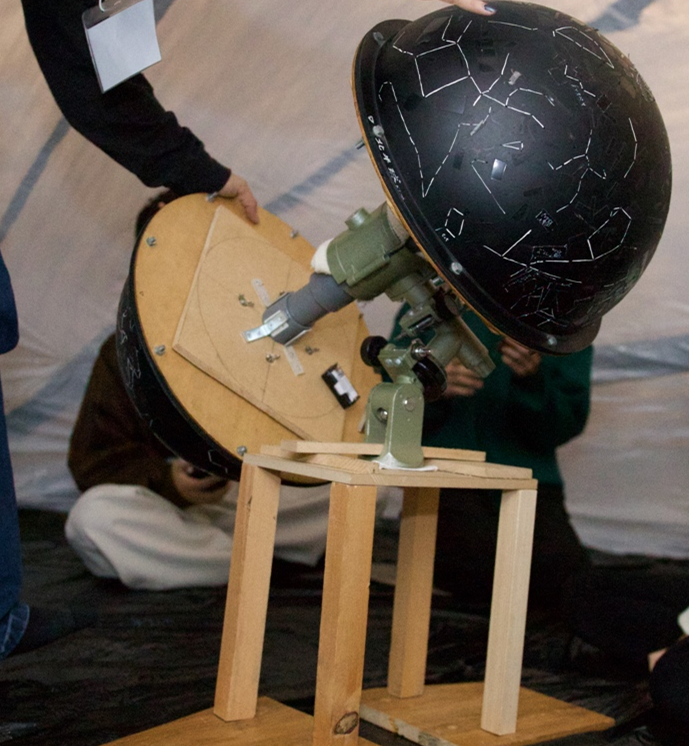
\includegraphics[width=8cm]{figures/Nakahara/fig1.png}
  \caption{{\footnotesize 去年まで実際に使っていたプラネタリウム、半球二つの隙間が大きく帯状の星がない部分ができてしまっていた。}}
  \label{fig:1}
\end{figure}

星は球面上に散らばっているように見えるので、球体の恒星球を作る場合は実際の星の位置のデータをもちいてその通りに恒星球に穴を開ければプラネタリウムが作れます。しかし、正二十面体の場合は、星の位置のデータから正二十面体のどの位置に穴を開ければいいかを映したい全ての星について計算する必要があります。穴を開ける位置を求めるための計算式を立てて、その計算式に基づいたプログラムを作成しコンピュータに計算してもらいました。

次に穴あけです。星にはそれぞれ明るさがあります。明るさは光量で決まるので、光量は面積に比例することを用いて、明るい星は穴の半径を大きく、暗い星は穴の半径を小さくします。星の明るさのデータも存在するため、それぞれの星をどのくらいの穴の大きさにすればいいか、先程の位置を求める時と同様に計算式を作り、それを元にプログラムを作成して計算しました。初めは開ける穴の大きさに最も近いドリルを用意して穴を開けていました。

\begin{figure}[H]
  \centering
  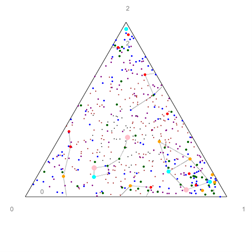
\includegraphics[width=8cm]{figures/Nakahara/fig2.png}
  \caption{\footnotesize ドリルで穴を開けるために作成していた画像、これを印刷して厚紙に貼り付け穴を開けていた。色ごとにドリルの刃の径を決めて穴あけ作業を行っていた。}
  \label{fig:2}
\end{figure}

一通り穴を開けたタイミングで、プラネタリウムの試し上映をしましたが、ここで問題が発生しました。穴は恒星球体の面に対して垂直に開けていたため、各面の端の方では、開けた穴に対して垂直に光が入らないため穴を通る光量が減り、面の重心から離れるにつれて星が暗くなってしまいました。その結果、三角形の面の中心部分は星がたくさんありますが端の方では星が全くないよう見えてしまいました。ドリルだけでは円形の穴しか開けられないため、穴の大きさを端の方では大きくすることで対処しようとしました。しかしここで、大学の設備でレーザーカッターを使えることがわかったため、それで穴を開けることにしました。円以外の形に穴を開けることも出来るため、穴の大きさを変えるのではなく、端の方の星は中心から外側に向かって引き伸ばしたような形に穴を開けることで明るさを保てます。レーザーカッターに読み込ませるための画像データを,計算した結果からプログラムで作成し、穴を開けました。ドリルの場合は用意した刃の径の種類分しか穴の大きさを変えられませんが、レーザーカッターの場合は好きな大きさで穴を開けられるので実際の星空により近づけられます。

\begin{figure}[H]
  \centering
  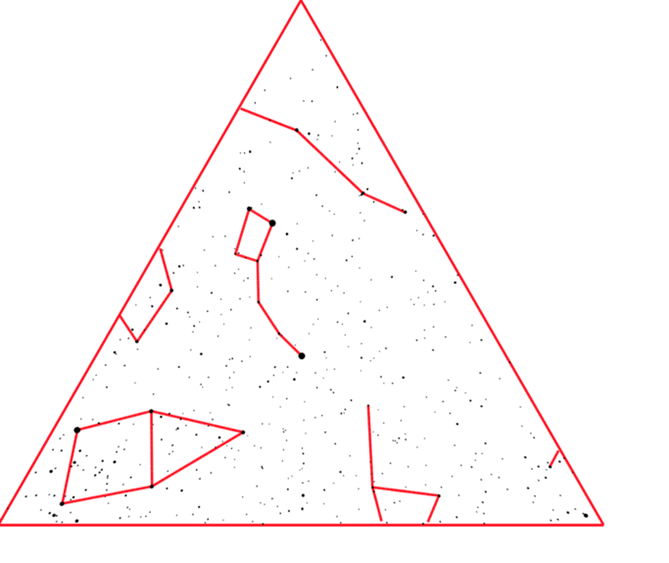
\includegraphics[width=8cm]{figures/Nakahara/fig3.png}
  \caption{\footnotesize レーザーカッターのために使用していた画像、よくみると端の方は綺麗な円でないことが確かめられる。}
  \label{fig:3}
\end{figure}

プラネタリウム制作を手伝ってくれた方々に感謝を述べてこの記事は終わりにしたいと思います。皆さんもぜひプラネタリウムを作ってみてください。私たちが作ったプラネタリウムを楽しんでくれると嬉しいです。

\begin{figure}[H]
  \centering
  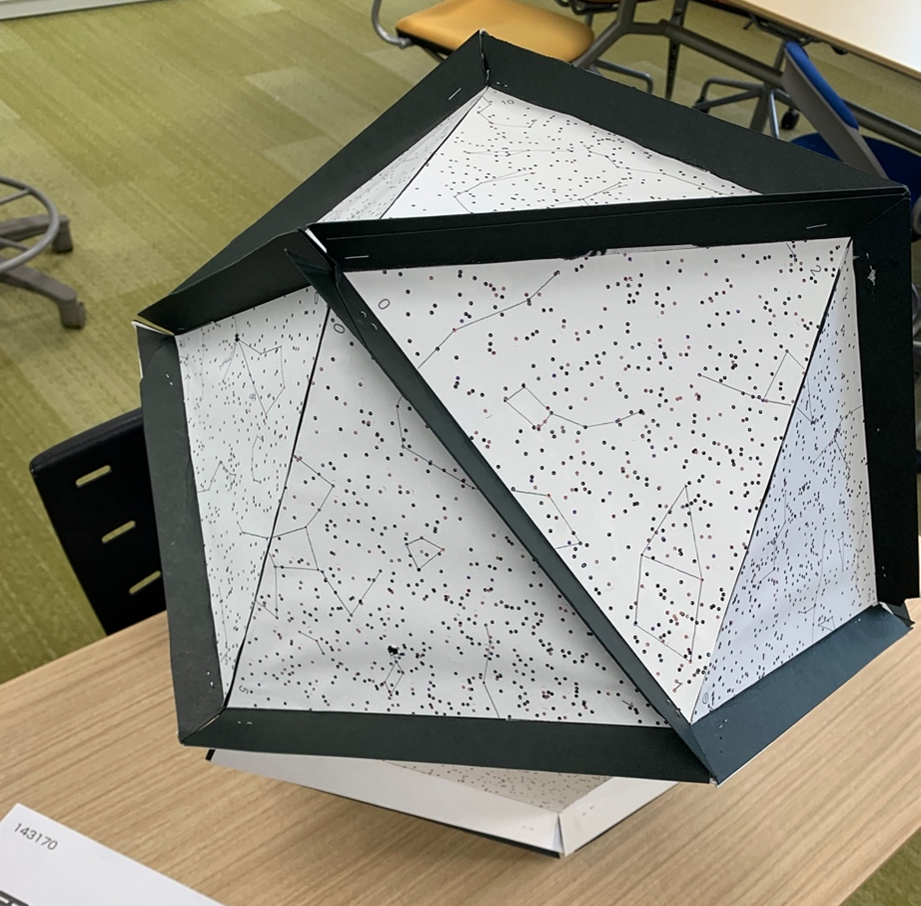
\includegraphics[width=8cm]{figures/Nakahara/fig4.png}
  \caption{\footnotesize 実際に正二十面体に組み立てた様子、部誌を書く段階ではレーザーカッターバージョンはまだ完成していないので試作品}
  \label{fig:4}
\end{figure}
\begin{figure}[H]
  \centering
  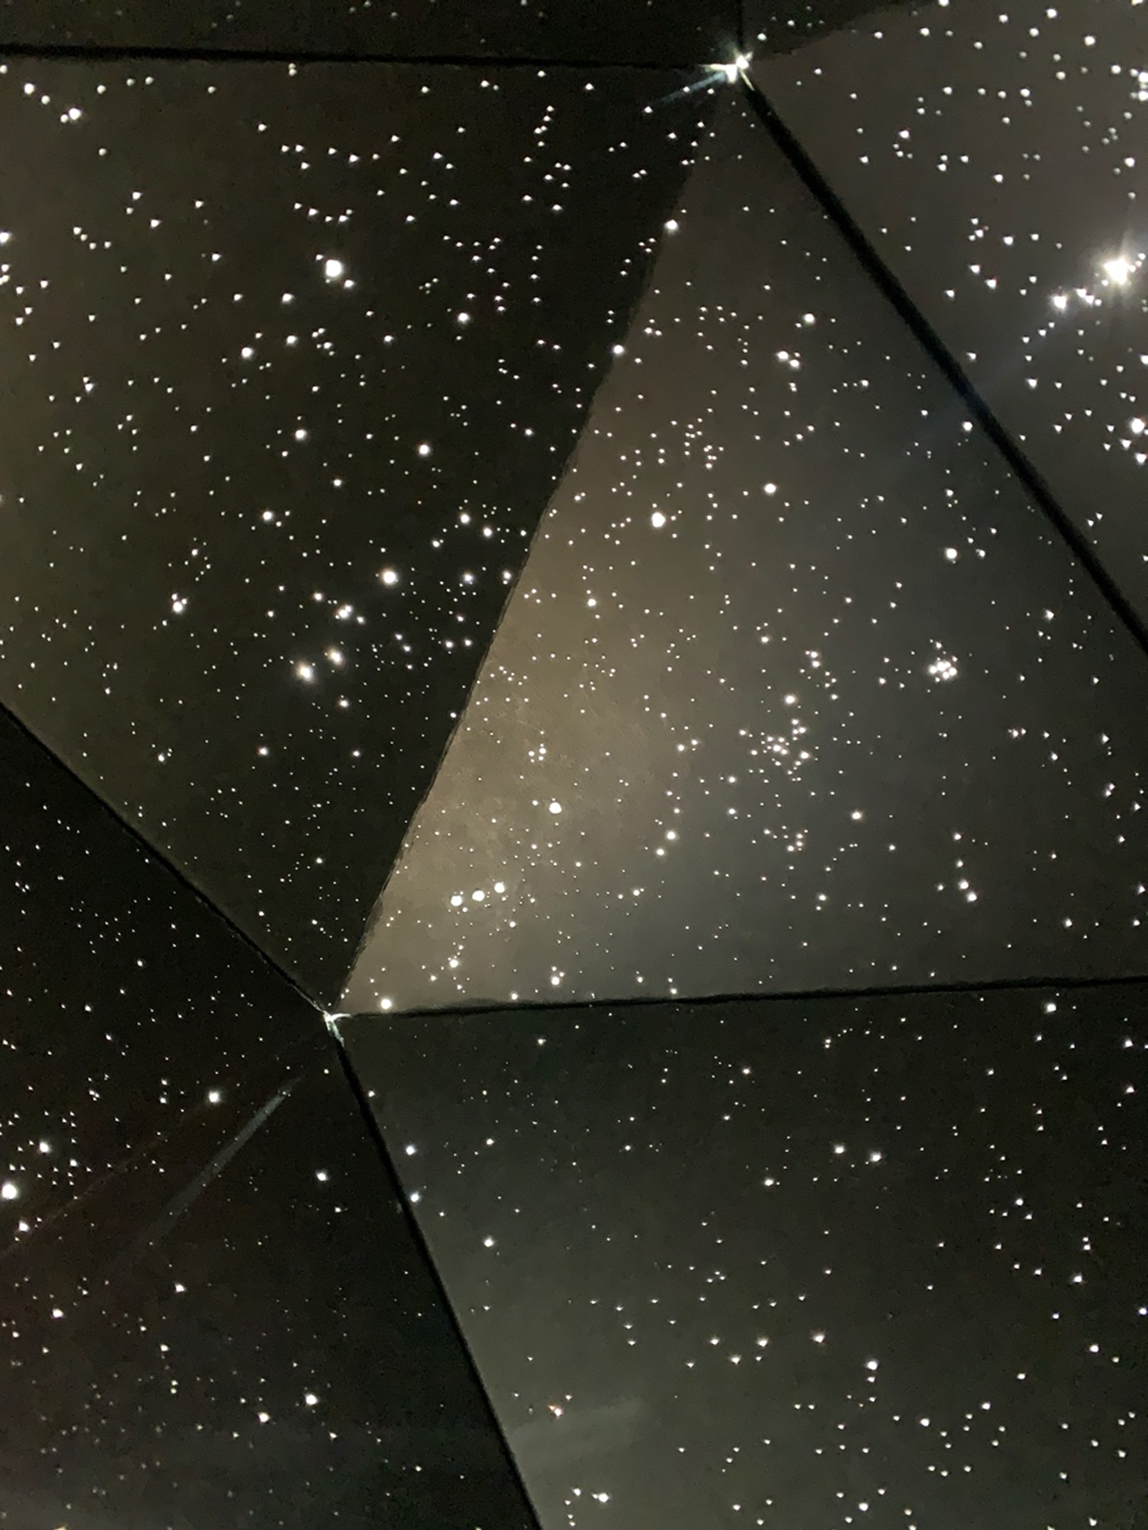
\includegraphics[width=8cm]{figures/Nakahara/fig5.png}
  \caption{\footnotesize 実は恒星球の中を覗くのが一番綺麗なのかもしれないと思う写真}
  \label{fig:5}
\end{figure}
\end{document}
